%!TeX root=../houndtop.tex
\chapter{Sir Henry Baskerville}
\lettrine[lines=4]{O}{ur} breakfast-table was cleared early, and Holmes waited in his dressing-gown for the promised interview. Our clients were punctual to their appointment, for the clock had just struck ten when Dr Mortimer was shown up, followed by the young baronet. The latter was a small, alert, dark-eyed man about thirty years of age, very sturdily built, with thick black eyebrows and a strong, pugnacious face. He wore a ruddy-tinted tweed suit and had the weather-beaten appearance of one who has spent most of his time in the open air, and yet there was something in his steady eye and the quiet assurance of his bearing which indicated the gentleman.

»This is Sir Henry Baskerville,« said Dr Mortimer.

»Why, yes,« said he, »and the strange thing is, Mr Sherlock Holmes, that if my friend here had not proposed coming round to you this morning I should have come on my own account. I understand that you think out little puzzles, and I've had one this morning which wants more thinking out than I am able to give it.«

»Pray take a seat, Sir Henry. Do I understand you to say that you have yourself had some remarkable experience since you arrived in London?«

»Nothing of much importance, Mr Holmes. Only a joke, as like as not. It was this letter, if you can call it a letter, which reached me this morning.«

He laid an envelope upon the table, and we all bent over it. It was of common quality, grayish in colour. The address, »Sir Henry Baskerville, Northumberland Hotel,« was printed in rough characters; the postmark »Charing Cross,« and the date of posting the preceding evening.

\begin{figure}[p]
\centering

\includegraphics[width=.8\linewidth]{04_sirhenry}
\caption{Sir Henry Baskerville}
\end{figure}

»Who knew that you were going to the Northumberland Hotel?« asked Holmes, glancing keenly across at our visitor.

»No one could have known. We only decided after I met Dr Mortimer.«

»But Dr Mortimer was no doubt already stopping there?«

»No, I had been staying with a friend,« said the doctor. »There was no possible indication that we intended to go to this hotel.«

»Hum! Someone seems to be very deeply interested in your movements.« Out of the envelope he took a half-sheet of foolscap paper folded into four. This he opened and spread flat upon the table. Across the middle of it a single sentence had been formed by the expedient of pasting printed words upon it. It ran: »As you value your life or your reason keep away from the moor.« The word »moor« only was printed in ink.

»Now,« said Sir Henry Baskerville, »perhaps you will tell me, Mr Holmes, what in thunder is the meaning of that, and who it is that takes so much interest in my affairs?«

»What do you make of it, Dr Mortimer? You must allow that there is nothing supernatural about this, at any rate?«

»No, sir, but it might very well come from someone who was convinced that the business is supernatural.«

»What business?« asked Sir Henry sharply. »It seems to me that all you gentlemen know a great deal more than I do about my own affairs.«

»You shall share our knowledge before you leave this room, Sir Henry. I promise you that,« said Sherlock Holmes. »We will confine ourselves for the present with your permission to this very interesting document, which must have been put together and posted yesterday evening. Have you yesterday's \textit{Times}, Watson?«

»It is here in the corner.«

»Might I trouble you for it—the inside page, please, with the leading articles?«  He glanced swiftly over it, running his eyes up and down the columns. »Capital article this on free trade. Permit me to give you an extract from it. »You may be cajoled into imagining that your own special trade or your own industry will be encouraged by a protective tariff, but it stands to reason that such legislation must in the long run keep away wealth from the country, diminish the value of our imports, and lower the general conditions of life in this island.« What do you think of that, Watson?« cried Holmes in high glee, rubbing his hands together with satisfaction. »Don't you think that is an admirable sentiment?«


Dr Mortimer looked at Holmes with an air of professional interest, and Sir Henry Baskerville turned a pair of puzzled dark eyes upon me.

»I don't know much about the tariff and things of that kind,« said he; »but it seems to me we've got a bit off the trail so far as that note is concerned.«

»On the contrary, I think we are particularly hot upon the trail, Sir Henry. Watson here knows more about my methods than you do, but I fear that even he has not quite grasped the significance of this sentence.«

»No, I confess that I see no connection.«

»And yet, my dear Watson, there is so very close a connection that the one is extracted out of the other. »You«, »your«, »your«, »life«, »reason«, »value«, »keep away«, »from the«. Don't you see now whence these words have been taken?«

»By thunder, you're right! Well, if that isn't smart!« cried Sir Henry.

»If any possible doubt remained it is settled by the fact that »keep away« and »from the« are cut out in one piece.«

»Well, now—so it is!«

»Really, Mr Holmes, this exceeds anything which I could have imagined,« said Dr Mortimer, gazing at my friend in amazement. »I could understand anyone saying that the words were from a newspaper; but that you should name which, and add that it came from the leading article, is really one of the most remarkable things which I have ever known. How did you do it?«

%»I presume, Doctor, that you could tell the skull of a negro from that of an Esquimau?\footnote{The Inuit people of the circumpolar region.}«

»I presume, Doctor, that you could tell the skull of a negro from that of an Esquimau?«

»Most certainly.«

»But how?«

»Because that is my special hobby. The differences are obvious. The supra-orbital crest, the facial angle, the maxillary curve, the\longdash«

»But this is my special hobby, and the differences are equally obvious. There is as much difference to my eyes between the leaded bourgeois type of a \textit{Times} article and the slovenly print of an evening half-penny paper as there could be between your negro and your Esquimau. The detection of types is one of the most elementary branches of knowledge to the special expert in crime, though I confess that once when I was very young I confused the \textit{Leeds Mercury} with the \textit{Western Morning News}. But a \textit{Times} leader is entirely distinctive, and these words could have been taken from nothing else. As it was done yesterday the strong probability was that we should find the words in yesterday's issue.«

»So far as I can follow you, then, Mr Holmes,« said Sir Henry Baskerville, »someone cut out this message with a scissors\longdash«

»Nail-scissors,« said Holmes. »You can see that it was a very short-bladed scissors, since the cutter had to take two snips over »keep away«.«

»That is so. Someone, then, cut out the message with a pair of short-bladed scissors, pasted it with paste\longdash«

»Gum,« said Holmes.

»With gum on to the paper. But I want to know why the word »moor« should have been written?«

»Because he could not find it in print. The other words were all simple and might be found in any issue, but »moor« would be less common.«

»Why, of course, that would explain it. Have you read anything else in this message, Mr Holmes?«

\begin{figure}[tbh]
\centering

\includegraphics[width=.7\linewidth]{04_inchdetail}
\caption{Holding it only an inch or two from his eyes}
\end{figure}

»There are one or two indications, and yet the utmost pains have been taken to remove all clues. The address, you observe is printed in rough characters. But the \textit{Times} is a paper which is seldom found in any hands but those of the highly educated. We may take it, therefore, that the letter was composed by an educated man who wished to pose as an uneducated one, and his effort to conceal his own writing suggests that that writing might be known, or come to be known, by you. Again, you will observe that the words are not gummed on in an accurate line, but that some are much higher than others. »Life«, for example is quite out of its proper place. That may point to carelessness or it may point to agitation and hurry upon the part of the cutter. On the whole I incline to the latter view, since the matter was evidently important, and it is unlikely that the composer of such a letter would be careless. If he were in a hurry it opens up the interesting question why he should be in a hurry, since any letter posted up to early morning would reach Sir Henry before he would leave his hotel. Did the composer fear an interruption—and from whom?«

»We are coming now rather into the region of guesswork,« said Dr Mortimer.

»Say, rather, into the region where we balance probabilities and choose the most likely. It is the scientific use of the imagination, but we have always some material basis on which to start our speculation. Now, you would call it a guess, no doubt, but I am almost certain that this address has been written in a hotel.«

»How in the world can you say that?«

»If you examine it carefully you will see that both the pen and the ink have given the writer trouble. The pen has spluttered twice in a single word, and has run dry three times in a short address, showing that there was very little ink in the bottle. Now, a private pen or ink-bottle is seldom allowed to be in such a state, and the combination of the two must be quite rare. But you know the hotel ink and the hotel pen, where it is rare to get anything else. Yes, I have very little hesitation in saying that could we examine the waste-paper baskets of the hotels around Charing Cross until we found the remains of the mutilated \textit{Times} leader we could lay our hands straight upon the person who sent this singular message. Halloa! Halloa! What's this?«

He was carefully examining the foolscap, upon which the words were pasted, holding it only an inch or two from his eyes.

»Well?«

»Nothing,« said he, throwing it down. »It is a blank half-sheet of paper, without even a water-mark upon it. I think we have drawn as much as we can from this curious letter; and now, Sir Henry, has anything else of interest happened to you since you have been in London?«

»Why, no, Mr Holmes. I think not.«

»You have not observed anyone follow or watch you?«

»I seem to have walked right into the thick of a dime novel,« said our visitor. »Why in thunder should anyone follow or watch me?«

»We are coming to that. You have nothing else to report to us before we go into this matter?«

»Well, it depends upon what you think worth reporting.«

»I think anything out of the ordinary routine of life well worth reporting.«

Sir Henry smiled.

»I don't know much of British life yet, for I have spent nearly all my time in the States and in Canada. But I hope that to lose one of your boots is not part of the ordinary routine of life over here.«

»You have lost one of your boots?«

»My dear sir,« cried Dr Mortimer, »it is only mislaid. You will find it when you return to the hotel. What is the use of troubling Mr Holmes with trifles of this kind?«

»Well, he asked me for anything outside the ordinary routine.«

»Exactly,« said Holmes, »however foolish the incident may seem. You have lost one of your boots, you say?«

»Well, mislaid it, anyhow. I put them both outside my door last night, and there was only one in the morning. I could get no sense out of the chap who cleans them. The worst of it is that I only bought the pair last night in the Strand, and I have never had them on.«

»If you have never worn them, why did you put them out to be cleaned?«

»They were tan boots and had never been varnished. That was why I put them out.«

»Then I understand that on your arrival in London yesterday you went out at once and bought a pair of boots?«

%»I did a good deal of shopping. Dr Mortimer here went round with me. You see, if I am to be squire down there I must dress the part, and it may be that I have got a little careless in my ways out West. Among other things I bought these brown boots—gave six dollars\footnote{Approximately \textdollar 200 USD in 2023.} for them—and had one stolen before ever I had them on my feet.«

»I did a good deal of shopping. Dr Mortimer here went round with me. You see, if I am to be squire down there I must dress the part, and it may be that I have got a little careless in my ways out West. Among other things I bought these brown boots—gave six dollars for them—and had one stolen before ever I had them on my feet.«


»It seems a singularly useless thing to steal,« said Sherlock Holmes. »I confess that I share Dr Mortimer's belief that it will not be long before the missing boot is found.«

»And, now, gentlemen,« said the baronet with decision, »it seems to me that I have spoken quite enough about the little that I know. It is time that you kept your promise and gave me a full account of what we are all driving at.«

»Your request is a very reasonable one,« Holmes answered. »Dr Mortimer, I think you could not do better than to tell your story as you told it to us.«

Thus encouraged, our scientific friend drew his papers from his pocket, and presented the whole case as he had done upon the morning before. Sir Henry Baskerville listened with the deepest attention, and with an occasional exclamation of surprise.

»Well, I seem to have come into an inheritance with a vengeance,« said he when the long narrative was finished. »Of course, I've heard of the hound ever since I was in the nursery. It's the pet story of the family, though I never thought of taking it seriously before. But as to my uncle's death—well, it all seems boiling up in my head, and I can't get it clear yet. You don't seem quite to have made up your mind whether it's a case for a policeman or a clergyman.«

»Precisely.«

»And now there's this affair of the letter to me at the hotel. I suppose that fits into its place.«

»It seems to show that someone knows more than we do about what goes on upon the moor,« said Dr Mortimer.

»And also,« said Holmes, »that someone is not ill-disposed towards you, since they warn you of danger.«

»Or it may be that they wish, for their own purposes, to scare me away.«

»Well, of course, that is possible also. I am very much indebted to you, Dr Mortimer, for introducing me to a problem which presents several interesting alternatives. But the practical point which we now have to decide, Sir Henry, is whether it is or is not advisable for you to go to Baskerville Hall.«

»Why should I not go?«

»There seems to be danger.«

»Do you mean danger from this family fiend or do you mean danger from human beings?«

»Well, that is what we have to find out.«

»Whichever it is, my answer is fixed. There is no devil in hell, Mr Holmes, and there is no man upon earth who can prevent me from going to the home of my own people, and you may take that to be my final answer.« His dark brows knitted and his face flushed to a dusky red as he spoke. It was evident that the fiery temper of the Baskervilles was not extinct in this their last representative. »Meanwhile,« said he, »I have hardly had time to think over all that you have told me. It's a big thing for a man to have to understand and to decide at one sitting. I should like to have a quiet hour by myself to make up my mind. Now, look here, Mr Holmes, it's half-past eleven now and I am going back right away to my hotel. Suppose you and your friend, Dr Watson, come round and lunch with us at two. I'll be able to tell you more clearly then how this thing strikes me.«

»Is that convenient to you, Watson?«

»Perfectly.«

»Then you may expect us. Shall I have a cab called?«

»I'd prefer to walk, for this affair has flurried me rather.«

»I'll join you in a walk, with pleasure,« said his companion.

»Then we meet again at two o'clock. Au revoir, and good-morning!«

We heard the steps of our visitors descend the stair and the bang of the front door. In an instant Holmes had changed from the languid dreamer to the man of action.

»Your hat and boots, Watson, quick! Not a moment to lose!« He rushed into his room in his dressing-gown and was back again in a few seconds in a frock-coat. We hurried together down the stairs and into the street. Dr Mortimer and Baskerville were still visible about two hundred yards ahead of us in the direction of Oxford Street.

»Shall I run on and stop them?«

»Not for the world, my dear Watson. I am perfectly satisfied with your company if you will tolerate mine. Our friends are wise, for it is certainly a very fine morning for a walk.«

He quickened his pace until we had decreased the distance which divided us by about half. Then, still keeping a hundred yards behind, we followed into Oxford Street and so down Regent Street. Once our friends stopped and stared into a shop window, upon which Holmes did the same. An instant afterwards he gave a little cry of satisfaction, and, following the direction of his eager eyes, I saw that a hansom cab with a man inside which had halted on the other side of the street was now proceeding slowly onward again.

»There's our man, Watson! Come along! We'll have a good look at him, if we can do no more.«

\begin{figure}[p]
\centering
\includegraphics[width=\linewidth]{04_ourman}
\caption{There's our man, Watson!}
\end{figure}

At that instant I was aware of a bushy black beard and a pair of piercing eyes turned upon us through the side window of the cab. Instantly the trapdoor at the top flew up, something was screamed to the driver, and the cab flew madly off down Regent Street. Holmes looked eagerly round for another, but no empty one was in sight. Then he dashed in wild pursuit amid the stream of the traffic, but the start was too great, and already the cab was out of sight.

»There now!« said Holmes bitterly as he emerged panting and white with vexation from the tide of vehicles. »Was ever such bad luck and such bad management, too? Watson, Watson, if you are an honest man you will record this also and set it against my successes!«

»Who was the man?«

»I have not an idea.«

»A spy?«

»Well, it was evident from what we have heard that Baskerville has been very closely shadowed by someone since he has been in town. How else could it be known so quickly that it was the Northumberland Hotel which he had chosen? If they had followed him the first day I argued that they would follow him also the second. You may have observed that I twice strolled over to the window while Dr Mortimer was reading his legend.«

»Yes, I remember.«

»I was looking out for loiterers in the street, but I saw none. We are dealing with a clever man, Watson. This matter cuts very deep, and though I have not finally made up my mind whether it is a benevolent or a malevolent agency which is in touch with us, I am conscious always of power and design. When our friends left I at once followed them in the hopes of marking down their invisible attendant. So wily was he that he had not trusted himself upon foot, but he had availed himself of a cab so that he could loiter behind or dash past them and so escape their notice. His method had the additional advantage that if they were to take a cab he was all ready to follow them. It has, however, one obvious disadvantage.«

»It puts him in the power of the cabman.«

»Exactly.«

»What a pity we did not get the number!«

»My dear Watson, clumsy as I have been, you surely do not seriously imagine that I neglected to get the number? № 2704 is our man. But that is no use to us for the moment.«

»I fail to see how you could have done more.«

»On observing the cab I should have instantly turned and walked in the other direction. I should then at my leisure have hired a second cab and followed the first at a respectful distance, or, better still, have driven to the Northumberland Hotel and waited there. When our unknown had followed Baskerville home we should have had the opportunity of playing his own game upon himself and seeing where he made for. As it is, by an indiscreet eagerness, which was taken advantage of with extraordinary quickness and energy by our opponent, we have betrayed ourselves and lost our man.«

We had been sauntering slowly down Regent Street during this conversation, and Dr Mortimer, with his companion, had long vanished in front of us.

»There is no object in our following them,« said Holmes. »The shadow has departed and will not return. We must see what further cards we have in our hands and play them with decision. Could you swear to that man's face within the cab?«

»I could swear only to the beard.«

»And so could I—from which I gather that in all probability it was a false one. A clever man upon so delicate an errand has no use for a beard save to conceal his features. Come in here, Watson!«

He turned into one of the district messenger offices, where he was warmly greeted by the manager.

»Ah, Wilson, I see you have not forgotten the little case in which I had the good fortune to help you?«

»No, sir, indeed I have not. You saved my good name, and perhaps my life.«

»My dear fellow, you exaggerate. I have some recollection, Wilson, that you had among your boys a lad named Cartwright, who showed some ability during the investigation.«

»Yes, sir, he is still with us.«

»Could you ring him up?—thank you! And I should be glad to have change of this five-pound note.«

A lad of fourteen, with a bright, keen face, had obeyed the summons of the manager. He stood now gazing with great reverence at the famous detective.

\begin{figure}[tbph]
\centering
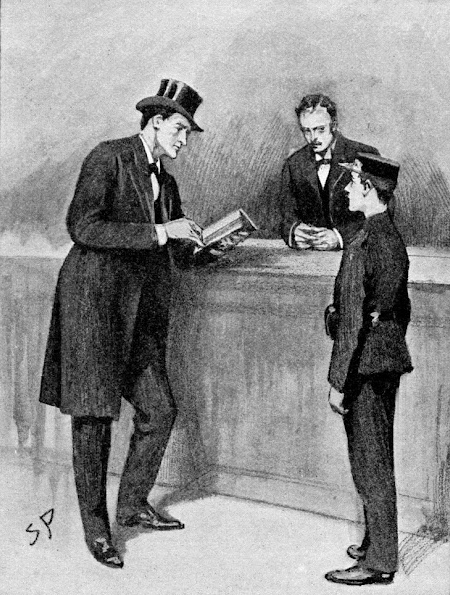
\includegraphics[width=\linewidth]{05_23hotels}
\caption{Here are the names of twenty-three hotels}
\end{figure}

»Let me have the Hotel Directory,« said Holmes. »Thank you! Now, Cartwright, there are the names of twenty-three hotels here, all in the immediate neighbourhood of Charing Cross. Do you see?«

»Yes, sir.«

»You will visit each of these in turn.«

»Yes, sir.«

»You will begin in each case by giving the outside porter one shilling. Here are twenty-three shillings.«

»Yes, sir.«

»You will tell him that you want to see the waste-paper of yesterday. You will say that an important telegram has miscarried and that you are looking for it. You understand?«

»Yes, sir.«

»But what you are really looking for is the centre page of the \textit{Times} with some holes cut in it with scissors. Here is a copy of the \textit{Times}. It is this page. You could easily recognize it, could you not?«

»Yes, sir.«

»In each case the outside porter will send for the hall porter, to whom also you will give a shilling. Here are twenty-three shillings. You will then learn in possibly twenty cases out of the twenty-three that the waste of the day before has been burned or removed. In the three other cases you will be shown a heap of paper and you will look for this page of the \textit{Times} among it. The odds are enormously against your finding it. There are ten shillings over in case of emergencies. Let me have a report by wire at Baker Street before evening. And now, Watson, it only remains for us to find out by wire the identity of the cabman, № 2704, and then we will drop into one of the Bond Street picture galleries and fill in the time until we are due at the hotel.«

\makeatletter
\@ifclasswith{scrbook}{a5paper}
{%
}{%
	\begin{figure}[p]
	\centering
	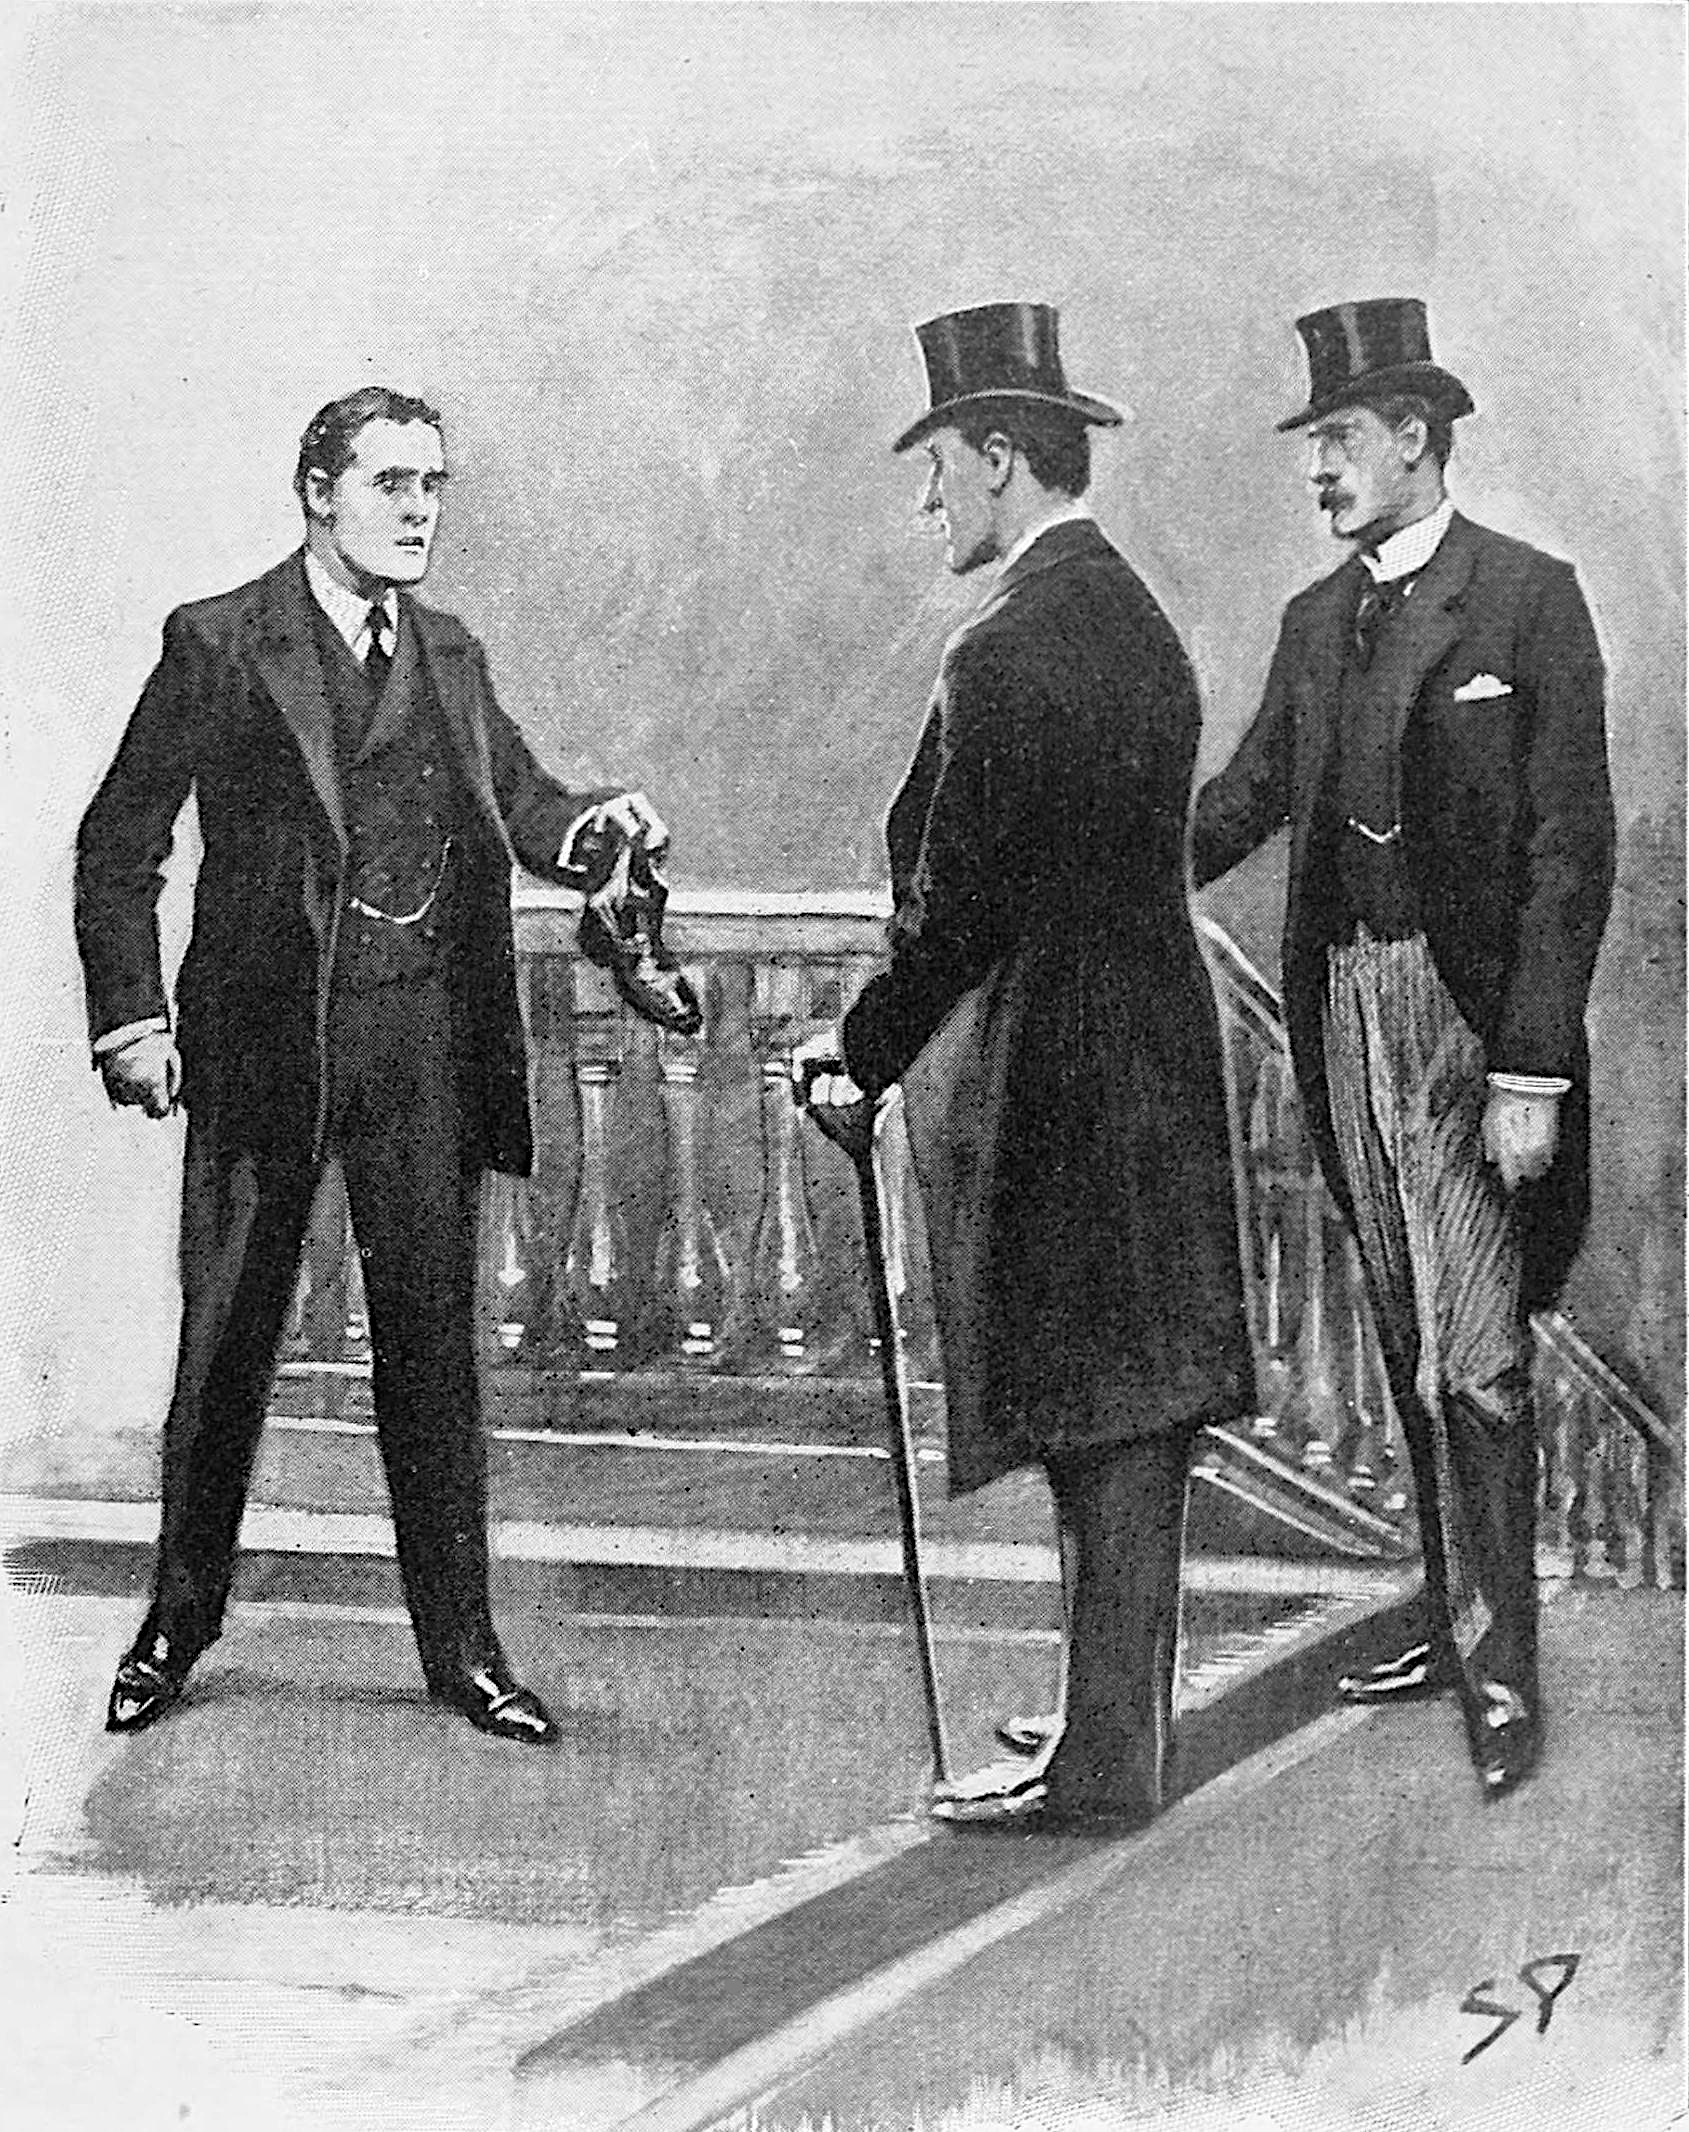
\includegraphics[width=\linewidth]{05_oldboot}
	\caption{He held an old and dusty boot in one of his hands}
	\end{figure}
}
\makeatother
